\section{Experimentální část}
\label{ExperimentalPart}
%% Program v C# pro analýzu + KNN a ANN + webová appka

%% ML.NET
%% .NET
%% Yara software
%% PeNet

%https://dotnet.microsoft.com/apps/machinelearning-ai/ml-dotnet

%% DONE:
%% VirusTotal
%% PE Reader
%% SEKCE
%% EP
%% STRINGS
%% HASHES
%% YARA
%% WEB
%% KONZOLE

%% TODO:
%%  PE Deep analysis
%%% Zdroje

%% NEURONKA

%% CO POUŽÍVÁM
%% co to umí
%% nějaké tesdty
%% porovnání?

%%%%%%%%%%%%%%
%%% ZACATEK TEXTU
%%%%%%%%%%%%%%

V rámci této práce byla implementována aplikace, jež provádí statickou analýzu požadovaného souboru se zaměřením na spustitelný formát \emph{Portable Executable} (viz kapitola \ref{pe_format}), a následně se pomocí strojového učení snaží testovaný vzorek klasifikovat. 

Pro vývoj byl zvolena platforma .NET framework. Motivací výběru tohoto frameworku, byla~možnost vývoje jak desktopové, tak webové aplikace. %% vyvíjeno jako knihovna zbytek je prostě jen vrstva nad tím

%%%%%%%%%%%%%%%% SUBKAPITOLA KNIHOVNY
\subsection{Použité nástroje a knihovny}
Při vývoji této aplikace bylo pro usnadnění jejího vývoje použito několik knihoven. Veškeré knihovny byly přidány do projektu pomocí správce balíčku službu určenou pro platformu .NET, NuGet. Tyto knihovny jsou popsány níže.

\paragraph*{PeNet}
%https://github.com/secana/PeNet
%Tato knihovna, jež umožňuje načíst a dále pracovat s PE souborem, je určena pro platformu v .NET. 
%C# (.NET)
%Native - žádné API cally atd.
\label{penet_lib}

PeNet je .NET knihovna, jež je určená pro parsování (což je syntaktická analýza) spustitelných souborů ve formátu PE (viz kapitola \ref{pe_format}) \cite{github_penet}. Tato knihovna je implementována ve standardizovaném formátu .NET Standard (viz \ref{dotnet_standard}). Je tady možné tuto knihovnu použít jak pro aplikace na Windows, tak například pro analýzu souboru v prostředí OS s jádrem Linuxu.

Tato knihovna umožňuje například extrakci jednotlivých části PE formátu, vytvoření otisku jednotlivých části jako jsou např. importy atd. A to bez jakékoliv závislosti na Windows API \cite{github_penet}. 

Knihovna má otevřený zdrojový kód a je dostupná pod licencí Apache 2.0. Může tak být použita v proprietárním softwaru \cite{github_penet}.

\paragraph*{VirusTotalNET}
%implementace API VirusTotal 2.0
% pro .NET
\label{virustotal_lib}

Pro práci s webovou aplikací VirusTotal, byla využita knihovna VirusTotalNET. Tato knihovna umožňuje spolupráci s API ve verzi 2 \cite{virustotal_net_lib}. 

VirusTotal umožňuje provedení analýzy jakéhokoliv souboru nebo url adresy. Služba obsahuje přes 70 antivirů, je tak skvělým nástrojem pro prvotní kroky analýzy \cite{virustotal_about}.

\paragraph*{ML.NET}
\label{ml_net}
Tato knihovna přidává nativní podporu strojového učení do frameworku \emph{.NET}, což umožňuje rozšířit jakoukoliv aplikaci na platformě \emph{.NET} o predikci stavu, detekování anomálií nebo třeba více třídní klasifikaci \cite{microsoft_mlnet}.

%TODO THIS?

\paragraph*{YARA}

YARA je nástroj určený pro identifikaci a klasifikaci vzorků primárně malwaru. Pomocí tohoto nástroje můžeme rozdělovat jednotlivé vzorky do skupin, a to na základě textových nebo binárních vzorů \cite{virustotal_yara}. 

Yara pracuje na principu vyhledávaní těchto vzorů dle předepsaných pravidel. Tato pravidla mohou obsahovat sadu řetězců nebo binárních dat. Pravidla si buď můžeme vytvořit sami nebo~použít jednu z dostupných otevřených databází. Poslední alternativou pak může být použití nástroje pro vygenerování těchto pravidel \emph{YarGen} \cite{Github_YaraGenerator}.

Následující příklad, prezentuje ukázkové pravidlo (viz výpis zdrojového kódu č. \ref{src:YaraExample}). První řádek definuje dané pravidlo jako \emph{Example} následně je pravidlo rozděleno do několika částí. V~našem případě \emph{meta}, \emph{strings} a \emph{condition}. První část \emph{meta} obsahuje metadata o tomto pravidlu, jako jsou například autor, popis apod. Část \emph{strings} obsahuje řetězce, které by měl testovaný vzorek obsahovat. V této části můžeme použít řetězec vyjádřený pomocí šestnáctkové soustavy, běžně vyjádřeného řetězce nebo regulární výraz. V poslední části se pak nachází podmínka, kterou musí testovaný vzorek splnit, aby pravidlo bylo vyhodnoceno pozitivně. V~našem případě musí vzorek obsahovat buď řetězec z proměnné \emph{\$text1} nebo \emph{\$text2}.

\noindent
\begin{minipage}[t]{1\textwidth}
    \lstinputlisting[basicstyle=\footnotesize,caption={Ukázka pravidla YARA},label=src:YaraExample]{zdrojaky/yara/example.yara}
\end{minipage}

%%% PRAVIDLO EXAMPLE

%%% PŘIDAT SKUPINY A EXAMPLE

%https://www.root.cz/clanky/reason-n-tice-zaznamy-a-uvod-do-pattern-matchingu/
%http://virustotal.github.io/yara/
%https://link.springer.com/chapter/10.1007/978-3-319-30481-6_26


\subparagraph*{Použití v .NET}

Pro použití nástroje YARA na platformě .NET bylo využito knihovny \emph{libyara.NET} vyvíjené společností \emph{Microsoft}, jež zajišťuje zjednodušené volání API pomocí adaptéru (angl. wrapper) knihovny libyara na platformě .NET \cite{github_yaradotnet}. 

\paragraph*{MIME}
\label{lib_mime}
Protože se nelze spoléhat pouze na příponu souboru. Bylo pro identifikaci typu souboru, využito standardu \emph{MIME} (zkr. Multipurpose Internet Mail Extensions). Tento standard byl původně navržen pro přílohy v emailové komunikaci. A obsahuje mimo jiné přesnou specifikaci názvu jednotlivých formátu.

%Obsahuje však jiné specifikaci formátu formátu souboru. 

Pro tento účel byla v .NET využita knihovna se stejným názvem \emph{MIME} \cite{libmagic_net}. Knihovna slouží jako adaptér pro knihovnu \emph{libmagic}, jež obsahuje databázi tzv. magických čísel (angl. magic numbers) viz kapitola \ref{magic_numbers}. Ty pak slouží k detekci formátu souboru \cite{libmagic_net}. Výstupem je pak standardizovaný název formátu souboru např. \emph{application/x-dosexec}, jež odpovídá spustitelnému souboru pro operační systém Windows nebo DOS.

%% umožňuje volání knihovny libmagic. 
%% https://github.com/ahupp/python-magic
%% https://github.com/hey-red/Mime
%% https://filemagic.readthedocs.io/en/latest/guide.html

%%%%%%%%%%%%%%%% SUBKAPITOLA Výstup aplikace

\subsection{Popis aplikace}
\label{process_analysis}

Vznikající program statické analýzy byl od začátku koncipován jako jednoduchá, modulárně rozšířitelná platforma, která bude umožňovat provedení přehledného výstupu. A to včetně případného automatického vyhodnocení testovaného vzorku pomocí knihovny ML.NET (viz kapitola \ref{ml_net}).

Architektura aplikace byla rozdělena do dvou vrstev viz obrázek č. \ref{fig:appLayers}. První vrstva zajišťuje veškeré prováděné kroky statické analýzy. Jako analýzu řetězců, přípravu výstupů apod. Tato~část byla vyvíjena ve specifikaci .NET standard, jež zajišťuje jednotnost chování programu na různých platformách \cite{dotnet_standard}. \label{dotnet_standard}
Druhá vrstva pak zajišťuje samotný výstup aplikace, v našem případě byla aplikace vyhotovena ve dvou provedeních. A to jako webová aplikace, tak jednoduchá konzolová aplikace. 

\begin{figure}[H]
    \caption{Jednotlivé vrstvy aplikace}
    \centering
    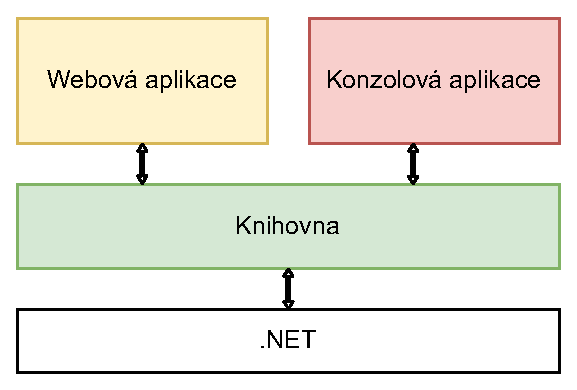
\includegraphics[width=95mm,scale=0.5]{Figures/obrazky/Programlayers.eps}
    \label{fig:appLayers}
\end{figure}

%Knihovna byla logicky rozvržena do několika částí. 

Průběh statické analýzy byl rozdělen do několika dílčích kroků. Jednotlivé kroky pak zabezpečují samotné moduly programu, kterých bylo v této práci vytvořeno celkem sedm.

Každý konkrétní modul provádí samostatný proces a je zcela nezávislý na modulech ostatních. To umožňuje kdykoliv přidat nebo odebrat některý z těchto modulů a případně knihovnu rozšířit o moduly nové.

Všechny vytvořené moduly implementují přetíženou metodu \emph{ToString}, která následně umožňuje snazší práci s výstupem aplikace.

Některé často používané funkcionality pro práci s řetězci a kolekcemi jsou implementovány formou externích rozšíření.

\paragraph*{Moduly}
\label{modules_app}

Implementovány byly následující moduly. Pořadí popisu modulů pak odpovídá jednotlivým krokům statické analýzy.

\subparagraph*{MIME} 

Prvním krokem statické analýzy je detekce typu MIME. Tu zajišťuje knihovna \emph{MIME} viz kapitola \ref{lib_mime}.

Nejprve je vytvořena instance třídy pro zjištění tohoto typu a poté se zavolá potřebná metoda, jež slouží k zjištění typu.
 
\subparagraph*{Hashes}

Tento modul zajišťuje výpočet několika různých hašovacích funkcí, a to konkrétně MD5, SHA-1, SHA-256, SHA-384, SHA-512.
Tyto funkce slouží primárně pro možnost případného vyhledání vzorku v různých databázích malwaru.

Z veřejných databází lze využít například databázi \emph{Malshare.com}, případně již dříve zmíněný VirusTotal.

\subparagraph*{VirusTotal}

Dalším modulem je modul pro aplikaci VirusTotal, předání pak zajišťuje knihovna \emph{VirusTotalNET} (viz kapitola \ref{virustotal_lib}).

Zpracování a odeslání dat službě VirusTotal, je velmi jednoduché a to proto, že většinu funkční části zajišťuje samotná knihovna. 

Nejprve je vytvořena instance třídy \emph{VirusTotal}. Pro komunikaci se službou VirusTotal je zapotřebí mít vytvořený účet v této službě a zaregistrovat si vlastní API klíč (jedná se o klíč pro programovatelné rozhraní služby, jež slouží k autorizaci požadavků). V základním režimu je~možné odeslat k testování 4 požadavky za minutu a 1000 požadavků denně.

Pokud již byla vytvořena instance, může následovat testování daného vzorku. Nejprve je~provedeno vyhledání v databázi již existujících výsledků testů. Pokud vzorek testován dosud nebyl, je odeslán k testu. Dalším omezením může být velikost souboru. Její horní hranice ve~veřejném API je 32 MB.

\subparagraph*{Entropie}

Následuje krok, ve kterém je vypočtena entropie pro zkoumaný soubor. Výsledek pak může naznačovat, zda bylo provedeno šifrování nebo komprese souboru \cite{sikorski2012practical}. 

V daném případě se provede výpočet pomocí následujícího vzorce \ref{vypocetEntropie}, který je aplikován na~načtený soubor v paměti jako pole bytů. 

\begin{equation}
    \label{vypocetEntropie}
    En=-\sum_{n=1}^{\infty} f_n * \frac{\log{f_n}}{\log{2}}
\end{equation}

\begin{equation}
    \label{vypocetEntropie_sub}
    f_n= \frac{p}{c}
\end{equation}

Kde $p =$ počet výskytu stejného bytu a $c =$ celková délka pole bytů.

Čím více se výsledná hodnota entropie ($En$) blíží číslu 8, tím více je pravděpodobné, že~se jedná o šifrovaný nebo komprimovaný soubor \cite{entropy}.

% vypočítám entropií
% což mi říká to a to blablablabla

Ukázku výsledné entropie prezentuje následující tabulka č. \ref{entropy_table}. Pro testování byl zvolen multimediální přehrávač VLC. Nejdříve bylo provedeno packování pomocí známého packeru pro kompresi UPX a komerečního packeru ASPack a následně byla vypočtena entropie jednotlivých souborů.

\begin{table}[H]
    \centering

    \begin{tabular}{|l|l|l|}
        \hline
            & Entropie & Velikost souboru \\ \hline \hline
         bez komprese   &   6.47 & 940 kB \\ \hline
         UPX            &   7.83 & 324 kB \\ \hline
         ASPack         &   7.85 & 316 kB \\ \hline
    \end{tabular}
    
    \caption{Ukázka entropie packerů UPX a ASPack}
    \label{entropy_table}
\end{table}

\subparagraph*{PE}

Modul PE zajišťuje analýzu hlavičky spustitelných souborů PE (viz kapitola č. \ref{pe_format}) a~to~za pomoci knihovny PeNET (viz kapitola \ref{penet_lib}).

Nejprve je generována instance třídy \emph{PeFile} z knihovny PeNET. Ta zajišťuje veškerou práci se strukturou PE souboru, jako jsou zjištění jednotlivých sekcí, importů knihoven, funkcí atd. 

Následně se pro zjednodušení práce s PE strukturou načtou do vlastní třídy modulu \emph{PE} importy, exporty, directories a sekce (viz kapitola \ref{pe_format}).

Modul obsahuje implementaci pro zjištění jak základních parametrů jako je adresa vstupního bodu (angl. entry point) programu, velikost, čas vytvoření, typ a zda se jedná o knihovnu DLL, ovladač nebo EXE soubor. Ale také pokročilejší informace o importovaných a exportovaných funkcích a knihovnách, seznam sekcí a jejich parametrů nebo seznam jednotlivých directories. 

Ukázku výstupu lze vidět na následujícím obrázku \ref{fig:consolePeResult}.

\begin{figure}[H]
    \caption{Ukázka výstupu informací o spustitelném souboru formátu PE}
    \centering
    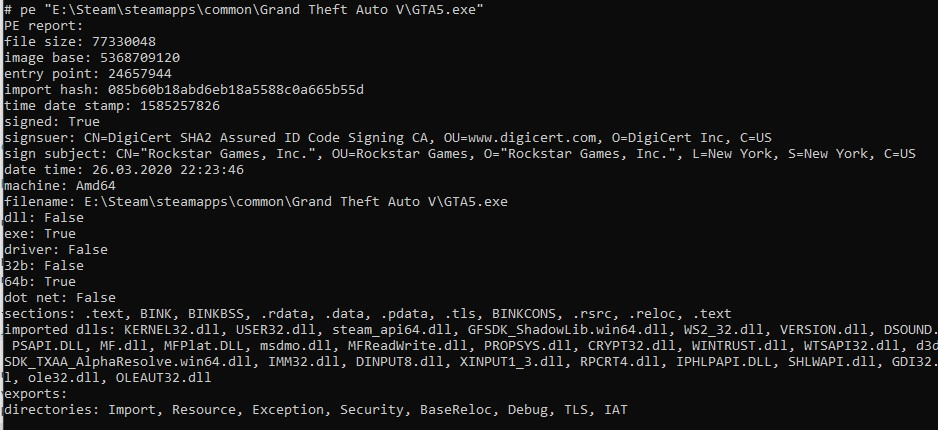
\includegraphics[width=160mm,scale=0.5]{Figures/obrazky/konzole-pe.jpg}
    \label{fig:consolePeResult}
\end{figure}

% co zkoumám
% co k tomu používám
% co si ukládám
% co mě zajimá

\subparagraph*{Strings}

Analýza řetězců probíhá v modulu \emph{Strings}. Průběh analýzy je rozdělen do několika kroků.
Nejprve je načten soubor do paměti a převeden na řetězec.
Poté je provedena filtrace nepožadovaných znaků (netisknutelné znaky, konec řetězce atp.), tyto znaky jsou odstraněny z toho důvodu, aby byla zajištěna lepší čitelnost výstupu při ruční analýze.

Následně je vyhledán název souborů uložených v programu pomocí vygenerovaného regulárního výrazu. Ten je vytvořen na základě získaného seznamu MIME typů (přípon souboru). Tento seznam je nejdříve načten do paměti z JSON souboru. Poté je provedeno vygenerování regulárního výrazu \emph{..(.jpg|.png ... |.exe)..} a vytvořena instance pro vyhledání jednotlivých výskytů v testovaném souboru. Zjištěná data jsou vrácena formou seznamu.

Dále je provedeno vyhledání důležitých informací, které mohou sloužit malwaru jako způsob, jak informovat útočníka o stavu útoku nebo naopak jako zdroj úkolu pro program, například vzdálená aktivace DDoS (Denial of service - útok s cílem zahltit požadovaný cíl) apod. Konkrétně se může jednat o IP adresy, emaily nebo informace ve formátu URL adresy jako \emph{https://}, \emph{smb://} nebo například \emph{ftp://}.

Vyhledání těchto dat se opět provádí pomocí regulárního výrazu, v tomto případě se pak jedná o předem vytvořené a uložené konstanty.

Posledním krokem analýzy je vyhledání známých metod používaných malwarem. Jako je například volání Windows API, Anti-debuggování atd. Seznam těchto metod byl získán z GitHub repositáře \emph{Cisco-Talos/Bass}. Vyhledání těchto metod je prováděno pomocí metody \emph{Contains}. Pokud je požadovaný řetězec obsažen, přidá se do seznamu.

% co zkoumám a jak
% zajimavosti o tom

\subparagraph*{Detect with Yara}

Pro detekci dalších vlastností byl vytvořen modul, který zajišťuje analýzu pokročilejších vlastností jako například kontrolu signatur různých packerů, výskyt různých metod chování na základě obsažené kombinace knihoven nebo detekci obranných mechanismů vůči analýze.

Pro tuto detekci, jsou použity již vytvořená pravidla z veřejného repositáře \emph{Yara-rules/rules} na platformě pro sdílení GIT repositářů Github.

A jsou to konkrétně pravidla pro detekci důležitých vlastností jako například obrana vůči debuggování nebo virtuálnímu prostředí. Dále to pak jsou pravidla pro detekci známých signatur packerů nebo kompilátorů.

%%%%%%%%%%%%%%%%%%%%%%%%%%%%%%%%%%%%%%%%%%%
\subsection{Výstup aplikace}

Pro zajištění výstupu je v knihovně \emph{StaticAnalysisProject.Lib} implementována třída \emph{FileReport}. Třída \emph{FileReport} zajišťuje veškerou inicializaci instancí jednotlivých modulů a zpracování dat z~jednotlivých části statické analýzy testovaného vzorku.

Řešení pak obsahuje implementaci dvou odlišných přístupů pro výstup aplikace. A to jako webová nebo konzolová aplikace. Ty jsou popsány v následujícím textu.

\paragraph*{Konzolová aplikace}

Rozhraní konzolové aplikace je koncipováno jako interaktivní uživatelský příkazový řádek. Po spuštění aplikace je uživatel uveden do prostředí programu, kde pomocí zápisu textových příkazů může tuto aplikaci ovládat.

Příkazy v programu jsou uzpůsobeny tak, že je možné provést buď jednotlivé kroky statické analýzy pomocí modulů této aplikace (viz kapitola \ref{modules_app}), anebo provést kompletní analýzu a získat tak výstup.

Na následujícím obrázku č. \ref{fig:consoleAppResult} lze vidět výstup interaktivního prostředí konzolové aplikace.

\begin{figure}[H]
    \caption{Ukázka výstupu konzolové aplikace}
    \centering
    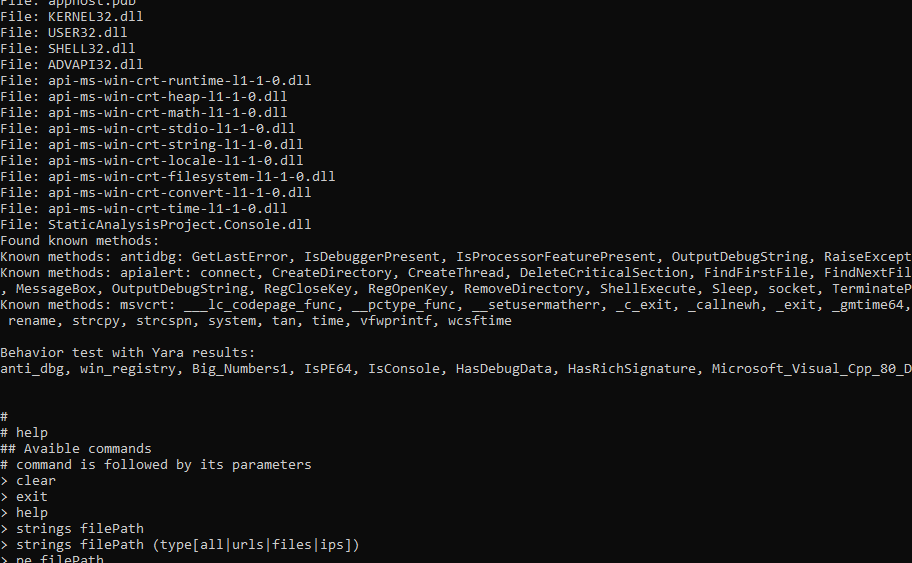
\includegraphics[width=160mm,scale=0.5]{Figures/obrazky/konzole.png}
    \label{fig:consoleAppResult}
\end{figure}

Další možností je pak spuštění aplikace s parametry, kdy lze získat přímý výstup bez nutnosti vstupovat do interaktivního prostředí programu.

\subparagraph*{Práce s aplikací}

Po spuštění se uživatel ocitne v interaktivním prostředí konzolové aplikace, kde může začít zadávat příkazy viz obrázek č. \ref{fig:consoleWork1}.

\begin{figure}[H]
    \caption{Práce s konzolovou aplikací - spuštění}
    \centering
    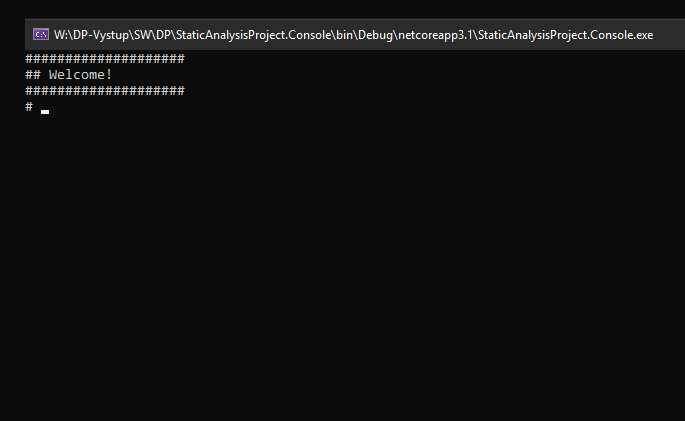
\includegraphics[width=135mm,scale=0.5]{Figures/obrazky/konzole-krok1.png}
    \label{fig:consoleWork1}
\end{figure}

Prvním příkazem, který může uživatel využít je příkaz \emph{help}, který zobrazí nápovědu (seznam použitelných příkazů) (viz obrázek č. \ref{fig:consoleWork2}).

\begin{figure}[H]
    \caption{Práce s konzolovou aplikací - příkaz help}
    \centering
    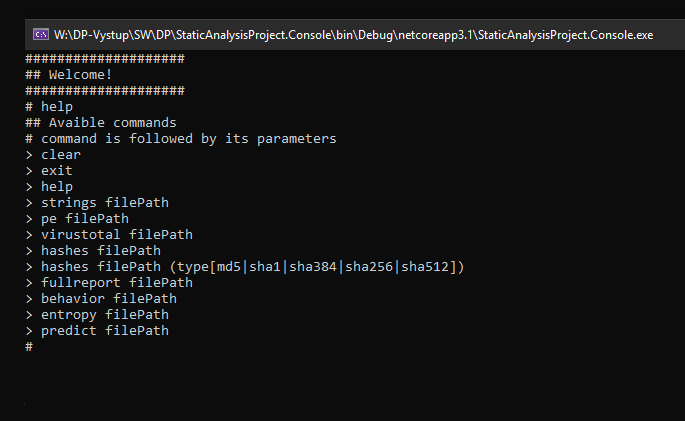
\includegraphics[width=135mm,scale=0.5]{Figures/obrazky/konzole-krok2.png}
    \label{fig:consoleWork2}
\end{figure}

Pokud je potřeba provést analýzu pomocí nástroje \emph{Yara}, použijeme příkaz \emph{behavior} viz obrázek č.~\ref{fig:consoleWork3}. Výstupem pak je seznam pozitivních pravidel, které mohou naznačovat chování aplikace. 

\begin{figure}[H]
    \caption{Práce s konzolovou aplikací - test pomocí Yara}
    \centering
    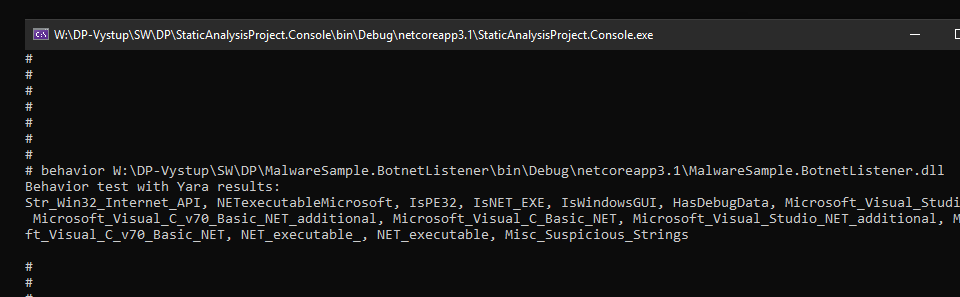
\includegraphics[width=135mm,scale=0.5]{Figures/obrazky/konzole-krok3.png}
    \label{fig:consoleWork3}
\end{figure}

Dalším příkazem pak může být testování službou \emph{VirusTotal}, která provede skenování různými antivirovými programy. Výstup lze vidět na obrázku č. \ref{fig:consoleWork4}

\begin{figure}[H]
    \caption{Práce s konzolovou aplikací - odeslání na VirusTotal}
    \centering
    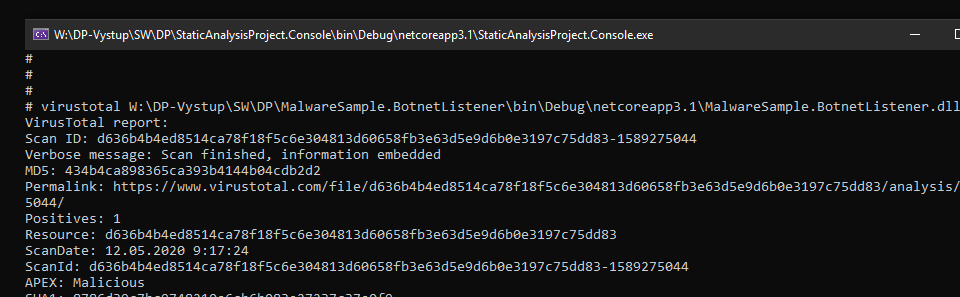
\includegraphics[width=135mm,scale=0.5]{Figures/obrazky/konzole-krok4.png}
    \label{fig:consoleWork4}
\end{figure}

\paragraph*{Webová aplikace}

Hlavním cílem vývoje webové aplikace, je možnost jednoduše bez nutnosti instalace dalšího softwaru provést statickou analýzu. 

Uživatelské rozhraní je velmi jednoduché, po otevření webové stránky v prohlížeči stačí zvolit požadovaný soubor. Následně je provedeno odeslání na webový server, kde je provedena statická analýza obdobně jako u konzolové aplikace s plným výstupem.

Uživatel tak může vidět kompletní výstup statické analýzy. Součástí výstupu je také výsledek binární klasifikace provedené pomocí knihovny ML.NET (viz kapitola \ref{ml_net}). Průběh klasifikace je popsán dále v kapitole \ref{app_testing}.

Při vývoji webové aplikace byly použity moderní technologie jako je framework jQuery, který umožňuje snazší vývoj interaktivních webových aplikací. Dále pak rozšíření standardních kaskádových stylů o dynamické funkce LESS a CSS framework Bootstrap ve verzi 4.

Na následujícím obrázku č. \ref{fig:webAppResult} je možné vidět ukázku výstupu webové aplikace. V první části je zvýrazněn výstup klasifikace, který byl dle predikované pravděpodobnosti barevně rozlišen (červená pokud je detekován malware; jestliže malware detekován nebyl a zároveň je pravděpodobnost vyšší než 80 \% je výsledek zobrazen zeleně; v případě, že je pravděpodobnost nižší než 80 \% je zvýrazněn žlutě; pokud má výsledek nižší pravděpodobnost než 20 \% je výsledek šedý).

\begin{figure}[H]
    \caption{Ukázka výstupu webové aplikace}
    \centering
    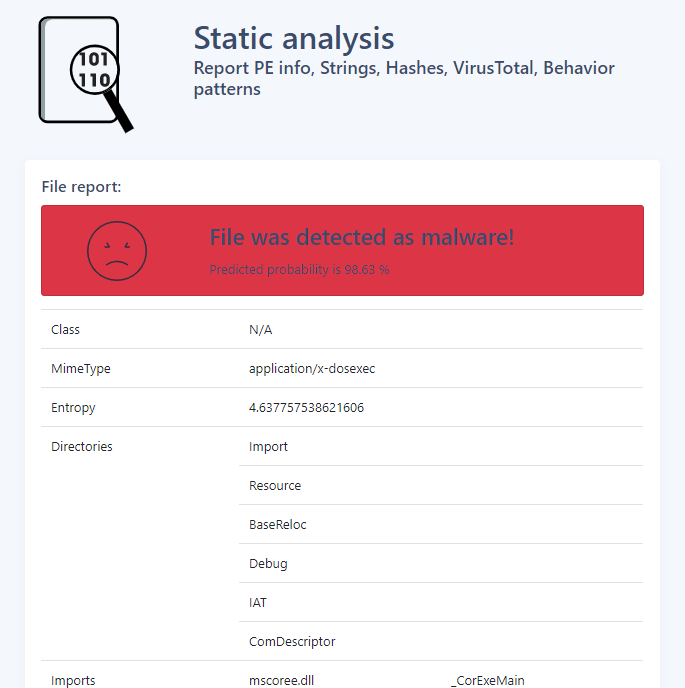
\includegraphics[width=135mm,scale=0.5]{Figures/obrazky/web.png}
    \label{fig:webAppResult}
\end{figure}

\subparagraph*{Práce s aplikací}

Po vstupu na webovou stránku je uživateli zobrazen webový formulář, kde je vyzván k výběru požadovaného souboru viz \ref{fig:workWithWebApp1}.

\begin{figure}[H]
    \caption{Práce s webovou aplikací krok 1.}
    \centering
    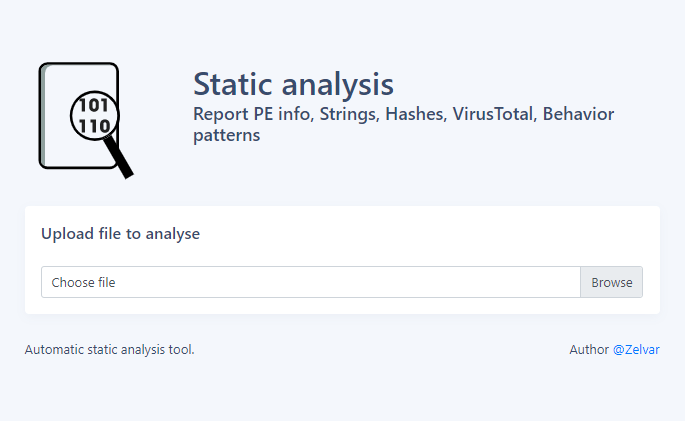
\includegraphics[width=135mm,scale=0.5]{Figures/obrazky/web-krok1.png}
    \label{fig:workWithWebApp1}
\end{figure}

Následně je vybrán požadovaný soubor pro testování viz obrázek č. \ref{fig:workWithWebApp2} a poté potvrzen výběr souboru.

\begin{figure}[H]
    \caption{Práce s webovou aplikací krok 2.}
    \centering
    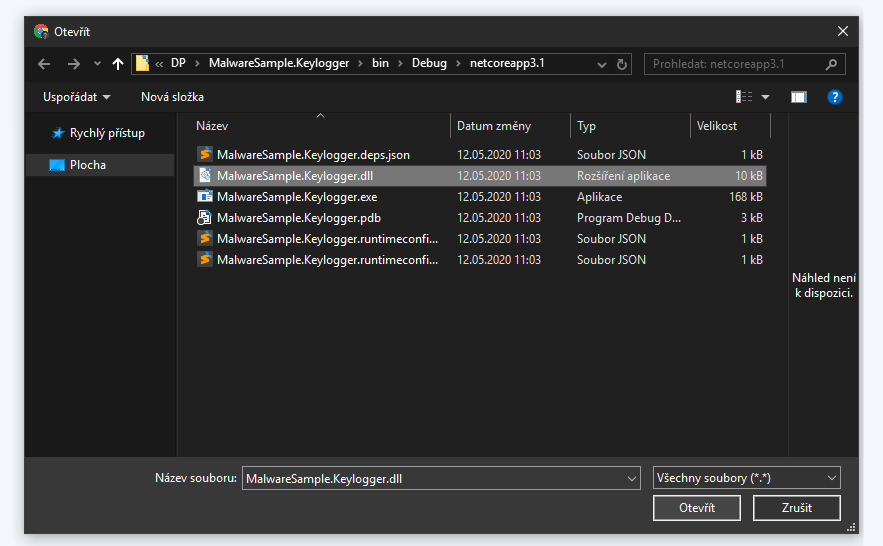
\includegraphics[width=135mm,scale=0.5]{Figures/obrazky/web-krok2.png}
    \label{fig:workWithWebApp2}
\end{figure}

Aplikace poté zpracuje analýzu požadovaného souboru a zobrazí ji uživateli, což je vidět na obrázku č. \ref{fig:workWithWebApp3}.

\begin{figure}[H]
    \caption{Práce s webovou aplikací krok 3.}
    \centering
    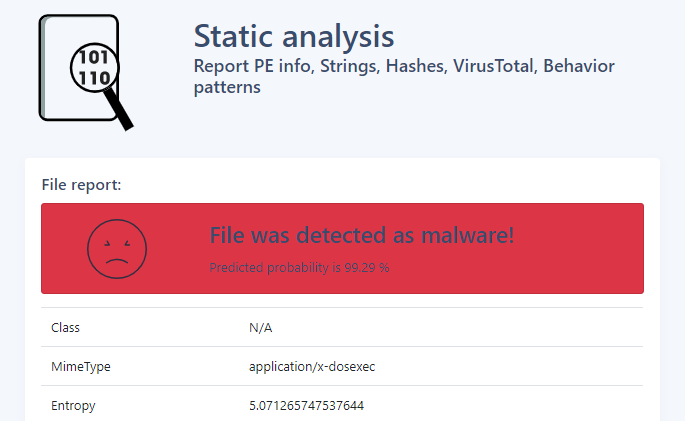
\includegraphics[width=135mm,scale=0.5]{Figures/obrazky/web-krok3.png}
    \label{fig:workWithWebApp3}
\end{figure}

%%%%%%%%%%%%%%%% SUBKAPITOLA Testování
\subsection{Testování aplikace}
\label{app_testing}

V průběhu vývoje programu byla aplikace testovaná na různých kategorií souborů. Především bylo testování zaměřeno na malware. Testování je pak konkrétněji popsáno dále v této kapitole.

%% TODO??
%\paragraph*{Porovnání s aplikacemi pro statickou analýzu}
%PeStudio atd?

\paragraph*{Testování malwaru}

%Za tímto účelem bylo z veřejně dostupných databází získán malware. Tento malware dále posloužil také jako vhodný zdroj informací pro vytvoření kolekce dat (angl dataset), jež měl sloužit jako zdroj informací pro strojové učení. 

Testování malwaru bylo prováděno formou analýzy zvolených souborů. Průběh této analýzy je zmíněn již v kapitole \ref{process_analysis}. Tato kapitola se dále zaměří pouze na testování malwaru určeného pro operační systém Windows ve formátu PE (viz kapitola \ref{pe_format}).

Aby analýza malwaru mohla být vůbec provedena, je nejprve zapotřebí vytvořit nebo získat vzorky malwaru. 

Za tímto účelem je z veřejně dostupných databází malwaru získáno 1952 vzorků, které jsou následně automaticky analyzovány pomocí vytvořeného programu. Tento malware také dále slouží jako vhodný zdroj informací pro vytvoření kolekce dat (angl. dataset), který má i funkci vstupního zdroje informací pro strojové učení. 

Již zmíněné databáze malwaru lze nalézt na webové adrese \url{https://dasmalwerk.eu} a~dále pak na GitHubu, konkrétně v repositáři \emph{ytisf/theZoo}.

Tak, aby bylo možné maximálně automatizovat skenování velkého množství dat, je vytvořen jednoduchý program. Tento program zajišťuje vyhledání souborů v požadované cestě určené při spuštění programu.

Program zároveň zajišťuje aby nedošlo k překročení omezení API služby \emph{VirusTotal}, která v základním tarifu nedovoluje více než 4 požadavky za minutu a 1000 požadavků za jeden den. V základním režimu je také omezena velikost souboru na 32 MB \cite{virustotal_limit}.

Nakonec se výsledky analýzy zaznamenávají do jednoho souboru ve formátu \emph{JSON}, který je~následně použit jako zdroj informací.

Pro porovnání bylo do datasetu také vloženo 108 výstupu legitimních aplikací (dále nazývané jako software). Při výběru je brán zřetel na nutnost různorodosti jednotlivých vlastností. Proto je vybráno několik podskupin jako například hry, správce souborů, kancelářské programy ale~také peněženky pro virtuální měny atd. Tato část kolekce je dále nazývána jako software.

%   U těchto vzorků bylo zjištěno ... STATISTIKA YARA + knihovny / fukce atd.
% https://docs.google.com/spreadsheets/d/1OwhYbQDeQnYJ14F48OLJ-BSLlGOWhqZMJ55G7Bl7-C8/edit#gid=0

%%%%%%%%%%%%%%%%%% STATS!!!!!!! TODO

Následující tabulka č. \ref{table:mimetypes_table} prezentuje podíl spustitelných souborů pro OS Windows, detekovaný pomocí modulu \emph{MIME} (viz kapitola \ref{modules_app}) obsažený v datové kolekci.

%application/x-dosexec
\begin{table}[H]
    \caption{Podíl spustitelných souborů v datasetu}
    \label{table:mimetypes_table}
    
    \centering
    \begin{tabular}{|l|l|l|}
        \hline
                            & Software & Malware       \\
        \hline
    	\hline
        PE (.exe, .dll)      & 108     & 769   \\ \hline
        jiný                 & 0       & 1183  \\ \hline
        celkem               & 108     & 1952  \\ \hline
    \end{tabular}
\end{table}

Vzhledem k tomu, že se práce zabývá primárně malwarem určeným pro operační systém Windows, jsou dále zohledňována a uváděna data pouze pro malware útočící právě na tento OS.

%%%%%%%%%% VLASTNOSTI PE
Tabulka č. \ref{table:pefile_table} demonstruje podíl jednotlivých parametrů spustitelných PE souborů v datové kolekci. Parametry \emph{16b}, \emph{32b} a \emph{64b} určují pro jakou architekturu procesoru je program určen, zda se jedná o 32 nebo 64 bitový systém. Vzhledem k tomu, že 64 bitový systém podporuje také spouštění 32 bitových aplikací. Útočnici mohou stále vytvářet škodlivý kód pro zajištění kompatibility s 32 bitovou verzí systému. Zároveň lze však dle statistik \emph{PassMark Software} očekávat sestupný podíl malwaru pro 32 bitovou platformu. A to převážně z důvodu klesajícího počtu instalací 32 bitových Windows \cite{passmark_32_stats}. 

Podíl podepsaného (Signed) škodlivého kódu nebo malwaru skrytého jako ovladače není často velký. Část nativního kódu převažuje nad kódem interpretovaným alespoň v případě platformy .NET.

\begin{table}[H]
    \caption{Parametry spustitelných souborů v kolekci dat}
    \label{table:pefile_table}
    
    \centering
    \begin{tabular}{|l|l|l|}
        \hline
               & Software & Malware \\ 
        \hline
        \hline
        16b    & 0.00 \%   & 1.56 \%  \\ \hline
        32b    & 50.00 \%  & 96.10 \% \\ \hline
        64b    & 50.00 \%  & 2.34 \%  \\ \hline
        DLL    & 21.30 \%  & 5.85 \%  \\ \hline
        EXE    & 78.70 \%  & 91.81 \% \\ \hline
        .NET   & 4.63 \%   & 15.08 \% \\ \hline
        Driver & 0.00 \%   & 0.13 \%  \\ \hline
        Signed & 33.33 \%  & 11.44 \% \\ \hline
    \end{tabular}
\end{table}

%%%%%%%%%%% SEKCE PE
Další tabulka č. \ref{table:sections_table} pak prezentuje střední hodnoty počtů sekcí spustitelných PE souborů v~jednotlivých skupinách. Na základě těchto dat lze usuzovat, že malware disponuje průměrně menším počtem sekcí než běžný software. 

\begin{table}[H]
    \caption{Počty sekcí v jednotlivých skupinách}
    \label{table:sections_table}
	
	\centering
	\begin{tabular}{|l|l|l|}
		\hline
		       & Software & Malware \\ 
		\hline
		\hline
		Průměr & 7.34     & 4.81    \\ \hline
		Medián & 7.00        & 4.00       \\ \hline
		S.D.   & 3.03     & 1.9    	\\ \hline
	\end{tabular}
\end{table}

%%%%%%%%%%%% Entropie graf + tabulka

\begin{table}[H]
    \caption{Entropie jednotlivých skupin}
    \label{table:entropie_table}
    
    \centering
	\begin{tabular}{|l|l|l|}
		\hline
		                    & Software & Malware \\
		\hline
		\hline
		Průměr              & 6.38     & 6.97                  \\ \hline
		Medián              & 6.41     & 7.08                  \\ \hline
		Směrodatná odchylka & 0.94     & 1.00                  \\ \hline
	\end{tabular}
\end{table}

Následující graf na obrázku č. \ref{fig:entropie} obsahuje četnosti hodnot entropie pro software a malware. Pro~lepší orientaci byla entropie zaokrouhlena v kroku 0.5. Hodnoty entropie softwaru vykazují na hladině spolehlivosti 98 \% normální rozložení naopak u hodnot entropie pro malware lze pozorovat extrém entropie v hodnotě 6.0 a druhý v hodnotně 8.0. Zároveň je z tabulky 9 patrné, že průměrné hodnoty entropie a také jejího mediánu jsou pro malware vyšší než pro software. To,~že~se~hodnoty statisticky významně liší, bylo prokázáno i za použití Mann-Whitneyova U-testu. 

\begin{figure}[H]
    \noindent
    \centering
    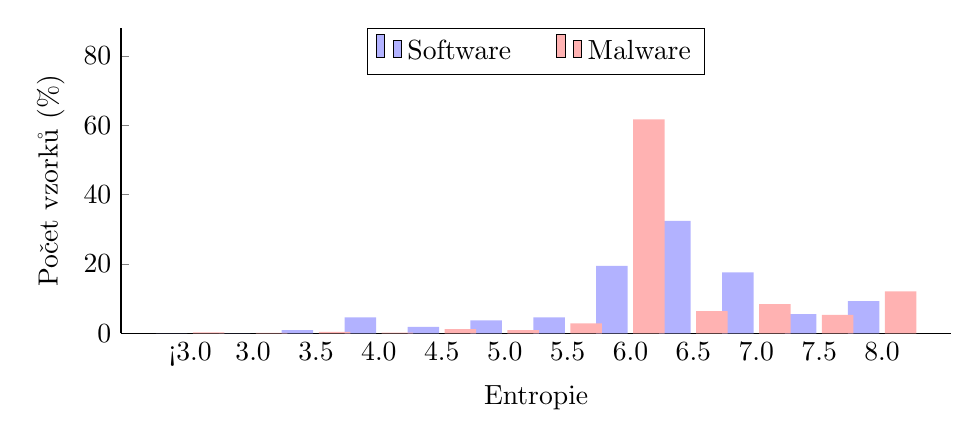
\begin{tikzpicture}
    \centering
    \begin{axis}[
                ybar,
                bar width=0.4cm, 
                width=\textwidth,
                height=.45\textwidth,
                ymajorgrids, tick align=inside,
                major grid style={draw=white},
                enlarge y limits={value=.1,upper},
                ymin=0, ymax=80,
                axis x line*=bottom,
                axis y line*=left,
                yminorgrids = true,
                y axis line style={opacity=100},
                tickwidth=0pt,
                enlarge x limits=true,
                legend style={
                    at={(0.5,1)},
                    anchor=north,
                    legend columns=-1,
                    /tikz/every even column/.append style={column sep=0.5cm}
                },
                minor ytick={0,20,...,100},
                grid=both,
                ylabel={Počet vzorků (\%)},
                xlabel={Entropie},
                symbolic x coords={<3.0,3.0,3.5,4.0,4.5,5.0,5.5,6.0,6.5,7.0,7.5,8.0},
               xtick=data,
               nodes near coords={
                %\pgfmathprintnumber[precision=0]{\pgfplotspointmeta}
               }
            ]
        \addplot [draw=none, fill=blue!30] coordinates {(<3.0, 0.00)(3.0, 0.00)(3.5, 0.93)(4.0, 4.63)(4.5, 1.85)(5.0, 3.70)(5.5, 4.63)(6.0, 19.44)(6.5, 32.41)(7.0, 17.59)(7.5, 5.56)(8.0, 9.26)};
        \addplot [draw=none, fill=red!30] coordinates {(<3.0, 0.26)(3.0, 0.15 )(3.5, 0.41 )(4.0, 0.20 )(4.5, 1.18 )(5.0, 0.92 )(5.5, 2.87 )(6.0, 61.73)(6.5, 6.40 )(7.0, 8.45)(7.5, 5.33)(8.0, 12.09)};
        \legend{Software, Malware}
    \end{axis}
    \end{tikzpicture}
    
    \caption{Entropie vzorků}
    \label{fig:entropie}
\end{figure}

%%%%%%%%%%% ŘETĚZCE

Dalším zjišťovaným parametrem (viz tabulka č. \ref{table:strings_table}) byla informace, jež určovala zda testovaný vzorek obsahuje konkrétní typ řetězce. V tomto případě se jednalo o \emph{email}, \emph{ip adresu} (jak IPv4 tak IPv6) a \emph{url adresu}. Zajímavým zjištěním je, že v případě malwaru je výskyt \emph{emailové} a~\emph{url} adresy nižší. V případě malwaru mohou tyto informace, které slouží často ke komunikaci s~útočníkem skryté pomocí různých obfuskačních metod viz kapitola \ref{obfuskacni_metody}. 

\begin{table}[H]
	\caption{Výskyt konkrétního typu řetězce}
	\label{table:strings_table}

    \centering
	\begin{tabular}{|l|l|l|}
	 	\hline
		     & Software & Malware \\
		\hline
		\hline
		Mail & 53.70 \%   & 26.80 \%  \\	 \hline
		IP   & 94.40 \%   & 87.30 \%  \\	 \hline
		URL  & 85.20 \%   & 34.30 \%  \\	 \hline
	\end{tabular}
\end{table}

%%%%%%%%%%% DLL
Následující data v tabulce č. \ref{table:libs_table} prezentují patnáct nejpoužívanějších knihoven v kolekci dat, používané jak softwarem tak malwarem. Na datech můžeme jasně vidět, že se použité knihovny se~velmi podobají a rozlišit malware od legitimních aplikací (software) pouze pomocí této informace není možné. Proto se tato informace kombinuje se seznamem použitých metod, které jsou volány z těchto knihoven. 

\begin{table}[H]
    \caption{Porovnání výskytu použitých knihoven}
    \label{table:libs_table}

    \centering
    \begin{tabular}{|l|l|l|l|}
        \hline
        \multicolumn{2}{|l|}{Software}                & \multicolumn{2}{|l|}{Malware} \\ \hline
        Knihovna                          & Výskyt  & Knihovna        & Výskyt    \\ 
        \hline
    	\hline
        kernel32.dll                      & 92.59 \% & kernel32.dll    & 76.98 \%   \\ \hline
        user32.dll                        & 75.00 \% & user32.dll      & 60.99 \%   \\ \hline
        advapi32.dll                      & 73.15 \% & advapi32.dll    & 59.82 \%   \\ \hline
        shell32.dll                       & 68.52 \% & gdi32.dll       & 38.75 \%   \\ \hline
        gdi32.dll                         & 57.41 \% & shell32.dll     & 36.80 \%   \\ \hline
        ole32.dll                         & 56.48 \% & ole32.dll       & 35.37 \%   \\ \hline
        oleaut32.dll                      & 44.44 \% & comctl32.dll    & 33.29 \%   \\ \hline
        comctl32.dll                      & 38.89 \% & oleaut32.dll    & 23.41 \%   \\ \hline
        version.dll                       & 37.96 \% & version.dll     & 21.07 \%   \\ \hline
        shlwapi.dll                       & 32.41 \% & ws2\_32.dll     & 19.25 \%   \\ \hline
        winmm.dll                         & 24.07 \% & mscoree.dll     & 14.95 \%   \\ \hline
        ws2\_32.dll                       & 22.22 \% & msvcrt.dll      & 14.95 \%   \\ \hline
        comdlg32.dll                      & 21.30 \% & shlwapi.dll     & 13.26 \%   \\ \hline
        vcruntime140.dll                  & 18.52 \% & wininet.dll     & 13.26 \%   \\ \hline
        api-ms-win-crt-runtime-l1-1-0.dll & 18.52 \% & comdlg32.dll    & 9.36 \%    \\ \hline
    \end{tabular}
\end{table}

%%%%%%%%% FUNKCE
Seznam patnácti nejpoužívanějších metod je pak možné vidět v následující tabulce č. \ref{table:methods_table}, kde je opět vidět jistou podobnost mezi softwarem a malwarem. Rozdíl ve volaných funkcích je však větší. Prvním příkladem může být metoda \emph{GetModuleHandleA}, kterou malware využívá k nalezení vhodného místa pro injekci vlastního kódu \cite{method_getmodulehandle}. Příkladem může být například injekce vlastního kódu do kernelu (\emph{GetModuleHandleA(kernel32.dll)}). Dalším metodou častěji používanou malwarem je \emph{LoadLibraryA}. Tato metoda slouží k dynamickému načtení modulu do~adresního prostoru aplikace. Často je také spolu s funkcí \emph{CreateRemoteThread} využívána při technice zvané \emph{DLL Injection} \cite{method_dllinjection}. Tato technika spočívá ve vložení (tzv. injekci) vlastního kódu do běžícího procesu. Tímto postupem může útočník injektovat malware například do procesů operačního systému. 

\begin{table}[H]    
    \caption{Porovnání výskytu použitých metod pro malware a software}
    \label{table:methods_table}
    
    \centering
    \begin{tabular}{|l|l|l|l|}
        \hline
        \multicolumn{2}{|l|}{Software}   & \multicolumn{2}{|l|}{Malware}   \\  \hline
        Funkce               & Výskyt  & Funkce              & Výskyt  \\
        \hline
    	\hline
        GetProcAddress       & 96.30 \% & GetProcAddress      & 81.79 \% \\ \hline
        CloseHandle          & 91.67 \% & WriteFile           & 67.75 \% \\ \hline
        GetCurrentThreadId   & 91.67 \% & GetModuleHandleA    & 65.54 \% \\ \hline
        GetLastError         & 91.67 \% & Sleep               & 64.63 \% \\ \hline
        Sleep                & 90.74 \% & CloseHandle         & 64.50 \% \\ \hline
        GetModuleHandleW     & 90.74 \% & GetLastError        & 63.20 \% \\ \hline
        QueryPerformanc..    & 89.81 \% & ExitProcess         & 62.03 \% \\ \hline
        GetCurrentProcess    & 89.81 \% & LoadLibraryA        & 59.17 \% \\ \hline
        WriteFile            & 87.96 \% & MultiByteToWideChar & 56.31 \% \\ \hline
        WideCharToMultiByte  & 87.04 \% & GetModuleFileNameA  & 52.15 \% \\ \hline
        MultiByteToWideChar  & 87.04 \% & GetTickCount        & 52.15 \% \\ \hline
        FreeLibrary          & 87.04 \% & WideCharToMultiByte & 49.80 \% \\ \hline
        UnhandledExcept..    & 83.33 \% & FreeLibrary         & 49.02 \% \\ \hline
        GetCurrentProcessId  & 81.48 \% & GetCurrentProcess   & 47.20 \% \\ \hline
        GetModuleFileNameW   & 80.56 \% & RegCloseKey         & 46.68 \% \\ \hline
        RegCloseKey          & 78.70 \% & VirtualAlloc        & 46.03 \% \\ \hline
        TerminateProcess     & 77.78 \% & WaitForSingleObject & 43.17 \% \\ \hline
        EnterCriticalSection & 77.78 \% & GetStdHandle        & 43.04 \% \\ \hline
        LeaveCriticalSection & 77.78 \% & ReadFile            & 42.91 \% \\ \hline
        GetSystemTimeAs..    & 76.85 \% & SetFilePointer      & 42.00 \% \\ \hline
    \end{tabular}
\end{table}


%%%%%%%%%%% YARA
Výskyt detekovaných pravidel prezentuje tabulka č. \ref{table:yara_table}. Na výsledných datech lze vidět procentuální výskyt patnácti nejčastějších pravidel, které byly detekovány v obou skupinách. V~případě malwaru můžeme jasně vidět, že bylo nejčastěji detekováno pravidlo (\emph{IsPE32}), které~detekuje 32 bitový spustitelný soubor ve formátu PE. Následují pravidla pro detekci výskytu grafického rozhraní pro Windows \emph{IsWindowsGUI} a pravidlo pro detekci manipulace s práce se soubory pomocí Windows API (\emph{win\_files\_operation}). Oproti běžnému softwaru, bylo u malwaru častěji detekováno pravidlo \emph{IsPacked}, které naznačuje, že u malwaru bylo detekován zabalení packerem (viz kapitola \ref{packers}). Dále pak bylo detekováno pravidlo \emph{SEH\_Init} a \emph{SEH\_Save}, které značí, že zdrojový kód aplikace obsahuje inicializaci pro strukturovanou obsluhu výjimek. V~tomto případě se může jednat o jeden ze způsobu ochrany proti ladění (anti-debug viz kapitola \ref{anti_debug}). Dalším důležitým pravidlem, které bylo detekováno je \emph{escalate\_priv}. Toto pravidlo detekuje způsoby jakým se útočník snaží získat vyšší oprávnění a to tak, aby bylo možné vykonat jinak nerealizovatelný útok \cite{privilage_escl}.

\begin{table}[H]
    \caption{Porovnání detekovaných YARA pravidel}
    \label{table:yara_table}
    
    \centering
    \begin{tabular}{|l|l|l|l|}
        \hline
        \multicolumn{2}{|l|}{Software}          & \multicolumn{2}{|l|}{Malware}                     \\ \hline
        Pravidlo              & Výskyt & Pravidlo                            & Výskyt \\ 
        \hline
        \hline
        IsWindowsGUI          & 75.00 \%       & IsPE32                              & 95.97 \%       \\ \hline
        win\_files\_operation & 64.81 \%       & IsWindowsGUI                        & 93.37 \%       \\ \hline
        HasOverlay            & 60.19 \%       & win\_files\_operation               & 58.00 \%       \\ \hline
        win\_registry         & 59.26 \%       & HasRichSignature                    & 56.18 \%       \\ \hline
        anti\_dbg             & 57.41 \%       & IsPacked                            & 52.93 \%       \\ \hline
        HasRichSignature      & 50.00 \%       & win\_registry                       & 44.21 \%       \\ \hline
        HasDebugData          & 50.00 \%       & SEH\_Init                           & 43.82 \%       \\ \hline
        IsPE32                & 45.37 \%       & HasOverlay                          & 36.02 \%       \\ \hline
        screenshot            & 42.59 \%       & screenshot                          & 33.29 \%       \\ \hline
        CRC32\_poly\_Constant & 42.59 \%       & CRC32\_poly\_Constant               & 30.43 \%       \\ \hline
        IsPE64                & 39.81 \%       & SEH\_Save                           & 29.78 \%       \\ \hline
        win\_token            & 37.04 \%       & MS\_VS\_Cpp\_v50..                  & 28.09 \%       \\ \hline
        win\_mutex            & 37.04 \%       & Str\_Win32\_Wins..                  & 27.05 \%       \\ \hline
        HasDigitalSignature   & 34.26 \%       & win\_token                          & 26.14 \%       \\ \hline
        keylogger             & 31.48 \%       & escalate\_priv                      & 22.11 \%       \\ \hline
    \end{tabular}
\end{table}

\paragraph*{Vlastní malware}
\label{own_malware_dp}

Pro účely testování jsou jako součást práce vytvořeny dva jednoduché druhy malwaru se zcela rozdílným vektorem útoku. Jednotlivé vlastnosti těchto škodlivých programů jsou popsány níže. Tyto vzorky byly primárně použity pro testování klasifikace. Výsledky těchto testů budou popsány dále.

Oba tyto testovací vzorky jsou implementovány v technologií .NET Core jako aplikace s~grafickým rozhraním (zkr. GUI) a to i přes to, že se při spuštění škodlivého programu žádné GUI nevytváří.

\subparagraph*{Botnet}

První ze dvou vzorků funguje na principu velmi jednoduchého klienta sítě, který je vzdáleně ovládán pomocí \emph{CnC} serveru. Klient může vykonávat pouze jednoduchý druh vyřadit službu z provozu (tzv. Denial of service), a to pomocí zasílání pingu z příkazového řádku. V~případě vytvoření větší sítě klientů by se pak mohlo jednat o distribuovaný druh útoku. Princip byl velmi zjednodušen s cílem vytvořit funkční imitaci malwaru. 

Celá síť se ovládá pomocí \emph{Command-and-Control} serveru, jež  byl implementován jako \emph{XML} (angl. Extensible Markup Language) dokument umístěný na webovém serveru. Tento dokument obsahuje cíl útoku (IP adresu) a informaci o aktivaci (zapnuto nebo vypnuto).

\subparagraph*{Keylogger}

Druhým škodlivým programem je pak aplikace pro skryté zaznamenávání stisku klávesnice a odesílání na webový server. Aplikace se po spuštění zavěsí na potřebné \emph{Windows API}, které slouží k získávání informací o stisku kláves a následně je vyvolávána při stisku volitelné klávesy událost, jež má za úkol zaznamenat stisknutý znak do proměnné. 

Pokud již bylo zaznamenáno 100 znaků, informace (zaznamenané stisky kláves) se odešlou na webový server, kde jej jednoduchý \emph{PHP} skript zaznamená do textového souboru.

V případě, že uživatel například použije platební kartu na internetu a útočník zaznamená jeho stisky kláves, mohou být jím zadané údaje následně zneužity.

%%%%%%%%%%%%%

\paragraph*{Klasifikace výstupu analýzy}

Klasifikace výstupu probíhala pomocí výše zmíněné technologie \emph{ML.NET} (viz kapitola \ref{ml_net}), která umožňuje snadné nasazení strojového učení na téměř jakoukoliv aplikaci.

Pro nasazení strojového učení stačí přidat do modelu, který obsahuje data, k jednotlivým proměnným parametr \emph{[LoadColumn(x)]} (kde \emph{x} je pořadí sloupce). Tím zajistíme možnost využít data pro strojové učení. Protože však technologie podporuje pouze některé datové typy (řetězce, boolean, float, vektorové data atd.) bylo potřeba data předzpracovat do požadovaného formátu. Proto byl model značně zjednodušen a obsahuje pouze některé parametry z výstupu statické analýzy.

Těmito parametry jsou základní vlastnosti PE hlavičky jako typ (Ovladač, \emph{DLL}, \emph{EXE}, platforma), zda je aplikace podepsaná digitálním certifikátem, třída (malware nebo software), entropie, detekované řetězce (\emph{email}, \emph{IP} a \emph{URL}), počet pozitivních testů \emph{VirusTotal}, seznam používaných metod a knihoven a zjištěné pozitivní výsledky pravidel \emph{Yara}.

Následně je provedeno automatické trénování (učení s učitelem) klasifikačního modelu pomocí vytvořené kolekce dat. Pro trénování je použito 80 \% dat datové kolekce, zbylých 30~\% je~použito pro křížovou validaci s deseti opakováními. Křížová validace má za úkol zjistit (vyhodnotit) jak moc jsou ovlivňovány nezávislé vzorky dat \cite{crossvalidation}.

Pro trénování byl použit algoritmus \emph{SdcaLogisticRegression}, který má zajistit dobré výsledky bez nutnosti jej dále ladit \cite{ms_mlnettraining}. Aby bylo možné tento algoritmus použít, je potřeba data nejdříve normalizovat. Pro tuto transformaci se využívá metoda \emph{NormalizeBinning}.

Součástí vypracovaní této diplomové práce je již vygenerovaný model na základě datové kolekce, která je také součástí. V případě však, že dojde ke změně dat je nutné tento model odstranit a nechat jej program vygenerovat znovu.

Následně se tento vytrénovaný model použije pro predikci třídy (software nebo malware), testovaného vzorku na základě výstupu statické analýzy.

\subparagraph*{Testování}
\label{my_malware_tests}

Pro testování byly použity výše zmíněné vzorky malwaru, které byly vytvořeny jako součást této práce (viz kapitola \ref{own_malware_dp}). A dvacet legitimních aplikací a dvacet dalších vzorků malwaru z databáze \emph{VirusShare.com}. Tyto vzorky nebyly použity při vytváření datové kolekce.

Následující tabulka č. \ref{table:my_malware} prezentuje výsledky testování vlastního malwaru. Jak lze vidět, malware byl detekován s přesností přes 90 \%. A oba vzorky byly pozitivně testovány. Úspěšnost je tedy 100 \%.

\begin{table}[H]
    \centering
    \begin{tabular}{|l|l|l|}
        \hline
        Soubor & Detekováno & Pravděpodobnost\\ \hline
        \hline
        KeyLogger.dll	&	Ano	&	91.34 \% \\ \hline
        BotnetListener.dll	&	Ano	&	93.71 \% \\ \hline
    \end{tabular}
    \caption{Detekce vytvořeného malwaru}
    \label{table:my_malware}
\end{table}

Další testování je provedeno na malwaru z databáze \emph{VirusShare.com}. Z této databáze je staženo 20 vzorků, které jsou podrobeny testům. Tabulka č. \ref{table:virusharae_malware} obsahuje část kontrolního součtu vytvořeného pomocí \emph{SHA-256} (kompletní kontrolní součty jsou pak součástí přílohy), název pod kterým byl detekován antivirem \emph{Avast}, zda byl detekován a s jakou pravděpodobnosti. V tomto případě je úspěšnost testování 100 \%.

\begin{table}[H]
    \centering
	\begin{tabular}{|l|l|l|l|}
		\hline
		SHA256    & Avast              			   & Detekováno & Pravděpodobnost \\ \hline
		\hline
		cbfc9d3.. & Undetected                     & Ano  & 99.99 \% \\ \hline
		8757088.. & Undetected                     & Ano  & 99.99 \% \\ \hline
		000ad60.. & Win32:PUP-gen {[}PUP{]}        & Ano  & 99.99 \% \\ \hline
		037bfec.. & Win32:AdwareSig {[}Adw{]}      & Ano  & 100 \% \\ \hline
		0872a6c.. & Win32:VBCrypt-AKV {[}PUP{]}    & Ano  & 99.99 \% \\ \hline
		190ea43.. & Win32:Downloader-GYZ {[}Trj{]} & Ano  & 99.99 \% \\ \hline
		1c757b4.. & Win32:Adware-CWL {[}PUP{]}     & Ano  & 99.32 \% \\ \hline
		21b0957.. & Win32:Adware-gen {[}Adw{]}     & Ano  & 99.99 \% \\ \hline
		2891ae4.. & Win32:Adware-gen {[}Adw{]}     & Ano  & 99.91 \% \\ \hline
		2e58e15.. & Win32:AdwareSig {[}Adw{]}      & Ano  & 99.99 \% \\ \hline
		436b7f2.. & Win32:Vundo-GZ {[}Trj{]}       & Ano  & 99.77 \% \\ \hline
		56bb2f5.. & Win32:AdwareSig {[}Adw{]}      & Ano  & 00.00 \% \\ \hline
		78c38d9.. & Win32:Dropper-OYB {[}PUP{]}    & Ano  & 99.99 \% \\ \hline
		97f1adc.. & Win32:AdwareSig {[}Adw{]}      & Ano  & 00.00 \% \\ \hline
		a2cb313.. & Win32:RmnDrp                   & Ano  & 99.81 \% \\ \hline
		abaa67c.. & Win32:AdwareSig {[}Adw{]}      & Ano  & 99.99 \% \\ \hline
		b154f80.. & Win32:AdwareSig {[}Adw{]}      & Ano  & 99.99 \% \\ \hline
		bf5b884.. & Win32:Mirc-AA {[}PUP{]}        & Ano  & 99.99 \% \\ \hline
		c494dab.. & Win32:Malware-gen              & Ano  & 99.98 \% \\ \hline
		db1ca5a.. & Win32:Malware-gen              & Ano  & 9.98 \%  \\ \hline
	\end{tabular}
    \caption{Detekce malwaru z databáze VirusShare.com}
    \label{table:virusharae_malware}
\end{table}

Poslední testování je provedeno nad sadou nepoužitých legitimních aplikací v datové kolekci. Výsledky tohoto testování prezentuje tabulka č. \ref{table:software_check}. V případě 3 vzorků (15 \% testů) dochází k predikcí tzv. \emph{false-positive} výsledku. Tento jev může být způsoben přecitlivělým predikčním modelem a bylo by vhodné datovou kolekci dále rozšířit.

\begin{table}[H]
    \centering
	\begin{tabular}{|l|l|l|l|}
		\hline
		SHA256    & Název souboru   			   & Detekováno & Pravděpodobnost \\ \hline
		\hline
		85601e9.. & Ozone Neon M50 Driver.exe      & Ano  & 99.05 \% \\ \hline
		9299fb2.. & Curse.exe                      & Ano  & 64.86 \% \\ \hline
		baf1879.. & Lanayo.VagrantManager.exe      & Ano  & 99.04 \% \\ \hline
		775a767.. & Amazon.Fuel.AppCore.dll        & Ne & 4.46 \%  \\ \hline
		dcdb065.. & CAMV2.Data.dll                 & Ne & 5.12 \%  \\ \hline
		459dd1e.. & EasyAntiCheat.exe              & Ne & 3.39 \%  \\ \hline
		47772a9.. & NeroPatentActivation.exe       & Ne & 4.79 \%  \\ \hline
		f2d6f5b.. & lua52.dll                      & Ne & 0.00 \%  \\ \hline
		c1c6c4c.. & mergecap.exe                   & Ne & 0.00 \%  \\ \hline
		280c0f7.. & obs32.exe                      & Ne & 0.00 \%  \\ \hline
		10effd4.. & OpenRL.dll                     & Ne & 0.00 \%  \\ \hline
		3ad5d5b.. & overlay.dll                    & Ne & 0.00 \%  \\ \hline
		b3e7e2e.. & phpstorm.exe                   & Ne & 40.39 \% \\ \hline
		4838635.. & python.exe                     & Ne & 0.05 \%  \\ \hline
		f4aae23.. & Qt5Core.dll                    & Ne & 0.00 \%  \\ \hline
		a64fe80.. & socialclub.dll                 & Ne & 0.00 \%  \\ \hline
		41229db.. & SocialClubHelper.exe           & Ne & 0.27 \%  \\ \hline
		a1a1372.. & trezord.exe                    & Ne & 0.04 \%  \\ \hline
		c67b7ac.. & java.exe                       & Ne & 0.12 \%  \\ \hline
		709bc7f.. & vulkaninfo.exe                 & Ne & 5.30 \%  \\ \hline
	\end{tabular}
    \caption{Detekce legitimních aplikaci}
    \label{table:software_check}
\end{table}

%vyběr algoritmu..
% https://github.com/dotnet/machinelearning/tree/master/docs

%Nejdříve byl proveden test pomocí zcela automatického módu \emph{AutoML}. 